%% Document coming from Julien Diot's Latex template.
%% This template is available on github:
%% https://github.com/juliendiot42/LatexTemplate
%% Please don't forget to cite this links if you use this template.
%%

%% Main tex file.






\documentclass[12pt,a4paper]{report}

% ========== Packages =========
% encoding and language:
\usepackage[utf8]{inputenc}  % UTF-8 encoding (recommended)
\usepackage[english]{babel}  % for english documents
%\usepackage[french]{babel}  % for french documents

% Math symbols:
\usepackage{amsmath}  % LaTeX library of American Mathematical Society useful macros
\usepackage{amssymb}  % To use math symbol
\usepackage{amsfonts} % To use math font
\usepackage{amsthm}   % Theorem, definition and proof

% figures / tables:
\usepackage{graphicx} % For graphic settings
\usepackage{float} % loating figures
\usepackage{tabularx} % auto size table
\usepackage{supertabular} % large tables
\usepackage{multirow} % table with cells on multiple row
\usepackage{listings} % For code part eg: \begin{lstlisting}[language=R] ..... \end{lstlisting}

% fonts :
\usepackage{xcolor}   % For color managment

% page layout:
\usepackage{fullpage} % Reduce margin for title page
\usepackage{fancyhdr} % En-têtes et pieds de pages
%\usepackage{lscape}   % use landscape pages
\usepackage{pdflscape} % use landscape pages (with pdfLatex)

% conditional expression in latex (example in "src/_abstract.tex")
\usepackage{ifthen}

% usefull package
\usepackage{lipsum} % lorem ipsum with "\lipsum[1-nParagraph]" command
\usepackage{comment} % To do comment on several lines with "\begin{comment} ... \end{comment}"
\usepackage{titling} % use \thetitle, \theauthor and \thedate
\usepackage{algorithmic} % easily write pseudo code. see: http://tug.ctan.org/macros/latex/contrib/algorithmicx/algorithmicx.pdf
\usepackage{enumitem} % personalised "bullet" list (use \begin{itemize}[label=\SymbToUse] )


% ========== Documents informations =========
\author{Julien Diot}
\title{Title of the document}
\date{\today}
%% Document coming from Julien Diot's Latex template.
%% This template is available on github:
%% https://github.com/juliendiot42/LatexTemplate
%% Please don't forget to cite this links if you use this template.
%%

%% Abstract definition
% this file define a new commande names "\myabstract"
% wich contain the abstract of the document in several languages.

\newcommand{\myabstract}[1][En]{
	\ifthenelse{\equal{En}{#1}}{
	Abstract in english...\\
	\lipsum[1]
	}{}
	\ifthenelse{\equal{Fr}{#1}}{
	Résumé en français...\\
	\lipsum[2]
	}{}
% add other language with:
%	\ifthenelse{\equal{OTHERLANG}{#1}}{
%	OTHERLANG...\\
%	\lipsum[2]
%	}{}
% ... 
} % the abstract are defined in an other file
						  % use "\myabstract[En]" to include your english abstract

\usepackage[pdftex]{hyperref} % use inlk and pdf informations
\hypersetup{
	bookmarks=true,         % show bookmarks bar?
	unicode=false,          % non-Latin characters in Acrobat’s bookmarks
	pdftoolbar=true,        % show Acrobat’s toolbar?
	pdfmenubar=true,        % show Acrobat’s menu?
	pdffitwindow=true,      % page fit to window when opened
	pdftitle={\thetitle},    % title
	pdfauthor={\theauthor},     % author
	% pdfsubject={subject of the document},   % subject of the document
	pdfnewwindow=true,      % links in new window
	pdfkeywords={Keyword1, Keyword2, ...}, % list of keywords
	colorlinks=true,       % false: boxed links; true: colored links
	linkcolor=black,          % color of internal links
	citecolor=black,        % color of links to bibliography
	filecolor=black,      % color of file links
	urlcolor=blue           % color of external links
}



%% ========== Document colors ==========
\definecolor{darkRed}{RGB}{92,0,2}
\definecolor{red}{RGB}{212,13,18}

\definecolor{darkGreen}{RGB}{25,68,41}
\definecolor{green}{RGB}{36,130,45}

\definecolor{darkBlue}{RGB}{9,27,66}
\definecolor{blue}{RGB}{49, 107, 179}

\definecolor{purple}{RGB}{179, 49, 172}
\definecolor{brown}{RGB}{179, 121, 49}



%% ========== image path ==========
\graphicspath{{src/img/}}
\newcommand{\logoExample}[1][0.12]{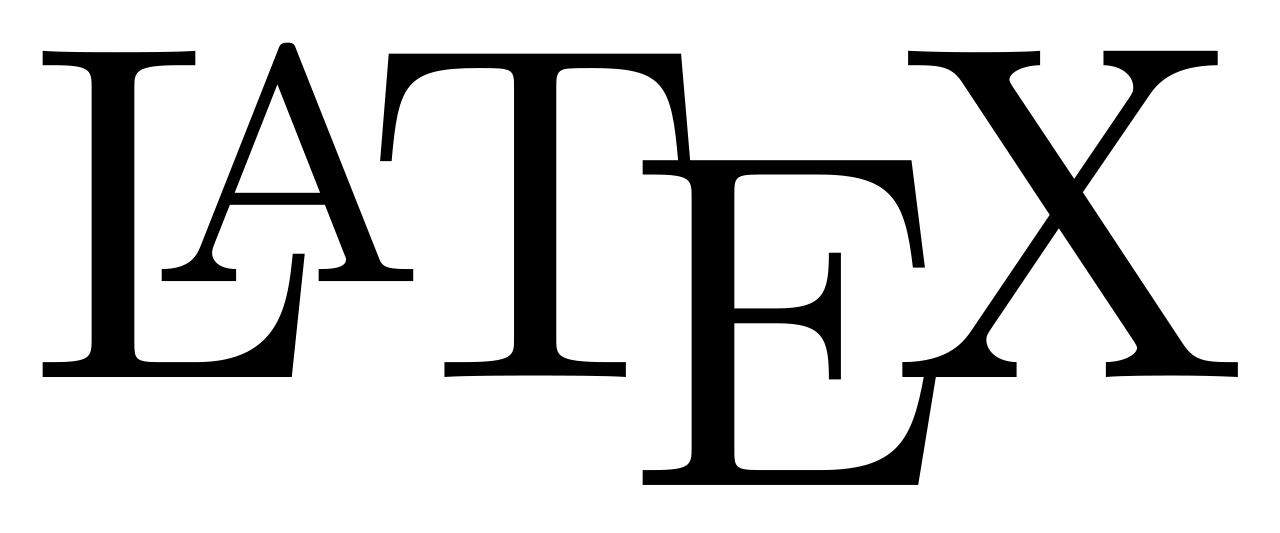
\includegraphics[scale={#1}]{logo_latex.png}}
%\newcommand{\myImg2}[1][0.5]{\includegraphics[scale={#1}]{image2.jpg}}



% ========== Layout ==========
\setlength{\parindent}{0pt} % paragraph indentation
\usepackage[left=2.cm,right=2.cm,top=2.5cm,bottom=2.5cm, headsep=5mm]{geometry} % Marges
\sloppy % do not cut word at the lines end



%% ========== Document structure ==========
\addto\captionsenglish{\renewcommand{\chaptername}{Part}} % rename "Chapter" to "Part"
\addto\captionsfrench{\renewcommand{\chaptername}{Partie}}% rename "Chapitre" to "Partie"

%% ========== Header and footer ==========

% redefine chapter name in normal case
%% header / footer for content pages:
\fancypagestyle{content}{%
	\fancyhead{} % reset footer
	\renewcommand{\headrulewidth}{0.4pt}
	\fancyhead[L]{\leftmark} % chaper name 
	\fancyhead[R]{\rightmark} % section name 
	
	\fancyfoot{} % reset footer
	\renewcommand{\footrulewidth}{0.4pt}
	\fancyfoot[L]{\theauthor\ - \textsc{A LaTeX Template.}}
	\fancyfoot[C]{CONTENT}
	\fancyfoot[R]{\thepage/\pageref{lastPage}}
}


%% header / footer for new chapter pages:
\fancypagestyle{plain}{%
	\fancyhead{} % reset footer
	\renewcommand{\headrulewidth}{0pt}
	
	\fancyfoot{} % reset footer
	\renewcommand{\footrulewidth}{0.4pt}
	\fancyfoot[L]{\theauthor\ - \textsc{A LaTeX Template.}}
	\fancyfoot[C]{PLAIN STYLE}
	\fancyfoot[R]{\thepage/\pageref{lastPage}}
}

%% header / footer for abstract / Appendix pages:
\fancypagestyle{abstractAppendix}{%
	\fancyhead{} % reset footer
	\renewcommand{\headrulewidth}{0pt}
	
	\fancyfoot{} % reset footer
	\renewcommand{\footrulewidth}{0.4pt}
	\fancyfoot[L]{\theauthor\ - \textsc{A LaTeX Template.}}
	\fancyfoot[C]{abstractAppendix}
	\fancyfoot[R]{\thepage}
}



%% ========== Lists ==========
% custom bullet style for lists:
\renewcommand{\labelitemi}{$-$}
\renewcommand{\labelitemii}{$\bullet$}
\renewcommand{\labelitemiii}{$\circ$}
%\renewcommand{\labelitemiv}{$\circ$}



%% ========== My macros ==========
% Math macro:
\newcommand{\N}{\mathcal{N}}% Normal distribution symb
\newcommand{\T}{\mathcal{T}}% Student distribution symb
\newcommand{\R}{\mathbb{R}} % Real number symb

% environment
\newenvironment{noteJD}
{\color{blue} \textit{Notes Julien: }}
{}

\newenvironment{note2}
{\color{darkRed} \textit{Notes style2: }}
{}

% ====================================================================================
% ====================================================================================
% ========== Begin document ==========
%
% 
\begin{document}


%% ==========  Title Page ========== 
%% Document coming from Julien Diot's Latex template.
%% This template is available on github:
%% https://github.com/juliendiot42/LatexTemplate
%% Please don't forget to cite this links if you use this template.
%%

%% Title page
% This page was inpired by Julien Enselme's title page see:
% https://www.jujens.eu/posts/2013/Oct/20/latex-page-garde/

% comand to create horizontal line
\newcommand{\Hline}[1][0.3]{\rule{\linewidth}{#1 mm}}


\begin{titlepage}
\enlargethispage{2cm}

  \begin{center}

	% 1st header 
    \textsc{\LARGE Main header on the top}\\[0.75cm]
    
	% second header
    \textsc{\Large
    Other header\\[0.5cm]
    on several lines}\\[1.5cm]

    % Title with horizontal lines
    \Hline \\[0.4cm]
    { \huge \bfseries  \thetitle \\[0.4cm] }
	\Hline \\[0.6cm]

    % Author and collaborators
	
    \begin{minipage}[t]{0.30\textwidth}
      \begin{flushleft} \large
        \emph{Author:} \theauthor \\
      \end{flushleft}
    \end{minipage}
    \begin{minipage}[t]{0.65\textwidth}
      \begin{flushright}
      {\large
        \emph{collaborators:}\quad\textsc{John Doe} {\normalsize(Status)}\\
        \textsc{Jane Doe} {\normalsize(Status)}\\
        \textsc{Johan Doe} {\normalsize(Status)}\\
        \vspace{0.5cm}
        
        \emph{Reviewer:}\quad\textsc{Mr. Smith}\\
        \vspace{0.5cm}
        
        \emph{Organization:}\quad\textsc{Latex Inc.}\\[0.5cm]
        
      }
      \end{flushright}
    \end{minipage}
    
    \vfill
    % Add some images here 
    \logoExample \hfill \logoExample
    
    \vfill
    
    
    
\end{center}

% Bottom : Date 
{\large  \thedate}

  

\end{titlepage}





%% ========== Abstract Page ==========
\clearpage
\pagestyle{abstractAppendix}

\pagenumbering{roman} % page number: i

\begin{center}
	\fbox{
		\begin{minipage}[t]{1 \textwidth}
		{\Large \textbf{Abstract:}}\\
		\myabstract[En]
		\end{minipage}
	}\\[2cm]

	\fbox{
		\begin{minipage}[t]{1 \textwidth}
		{\Large \textbf{Résumé :}}\\
		\myabstract[Fr]
		\end{minipage}
	}

\end{center}


% ========== TOC ==========
\clearpage
\tableofcontents
\thispagestyle{abstractAppendix}



% ========== Content ==========
\clearpage

%% reset page
\setcounter{page}{1} % reset page number
\pagenumbering{arabic} % and use arabic number

%% reset header / footer:
\pagestyle{content}
% re-def \chaptermark and \sectionmark
\renewcommand{\chaptermark}[1]{%
\markboth{\chaptername
\ \thechapter.\ #1}{}}
% redefine section name in normal case
\renewcommand{\sectionmark}[1]{\markright{\thesection.\ #1}}

%% soucre content files
%% Document coming from Julien Diot's Latex template.
%% This template is available on github:
%% https://github.com/juliendiot42/LatexTemplate
%% Please don't forget to cite this links if you use this template.
%%

%% Introduction


\chapter*{Introduction} % no number for introduction

%% add this chapter to the table of content:
\addcontentsline{toc}{chapter}{Introduction}


This is the introduction...\\

\lipsum[1-2]



%% Document coming from Julien Diot's Latex template.
%% This template is available on github:
%% https://github.com/juliendiot42/LatexTemplate
%% Please don't forget to cite this links if you use this template.
%%

%% Part one

\chapter{Example of some \LaTeX  commands}


\section{Insert references}
% how to instert 
First, fill the  bibTeX file (\texttt{.bib}) with your bibliography and place it in the same directory than your \texttt{main.tex} file.\\

You can then add  \verb=\cite{refKey}= in your text to insert a reference like this \cite{myRef1}.\\
The bibliography will be automatically filled.\\

The package \texttt{hyperref} will create some clickable links to the bibliography at the end of the document.


\section{Tables}

\subsection{With \texttt{tabular} }

\begin{tabular}{|l|c|r||c|l|r|}
\hline 
Col 1 & Col 2 & Col 3 & Larger column & \multicolumn{2}{c|}{People} \\ 
\hline 
a1 & b1 & c1 & d1 & GK & Guillaume Warmuz \\
a2 & b2 & c2 & d2 & LB & Yohan Lachor \\
a3 & b3 & c3 & d3 & DC & Jean-Guy Wallemme \\
\hline
\multirow{2}*{text}  & b4 & c4 & d4 & JD & Julien Diot \\
					 & b5 & c5 & d5 & JD & Julien Diot bis \\
\hline
\end{tabular}

\subsection{With \texttt{tabularx} }
% \begin{tabularx}{TableWidth}{|c|p{ColumnWidth}|X|}  X for autosize column
\begin{tabularx}{10cm}{|c|p{4cm}|X|}
    \hline
    1 & The two gentlemen of Verona & The Taming of the Shrew \\
    \hline
    2 & The comedy of errors & Love's Labour's Lost \\
    \hline
    3 & The Merchant of venice & The Merry Wives of Windsor \\
    \hline
\end{tabularx}



\begin{landscape}
\begin{center}

\section{Big table}


\tablefirsthead{
	\hline
	\multicolumn{1}{|c}{Number}
	& \multicolumn{1}{c}{Letters}
	& \multicolumn{1}{|c|}{Number!}\\
	\hline}
	
\tablehead{
	\hline
	\multicolumn{3}{|l|}{\small\sl continued from previous page}\\
    \hline
    \multicolumn{1}{|c}{Number}
	& \multicolumn{1}{c}{Letters}
	& \multicolumn{1}{|c|}{Number!}
	\\ \hline}
	
\tabletail{
	\hline
	\multicolumn{3}{|r|}{\small\sl continued on next page}\\
	\hline}
\tablelasttail{\hline}
\bottomcaption{This table is split across pages}
\par
\begin{supertabular}{| r @{\quad -sep- }| r@{\hspace{6 cm}}| r |}
One & abcdef ghjijklmn & 123.456778 \\
One & abcdef ghjijklmn & 123.456778 \\
One & abcdef ghjijklmn & 123.456778 \\
One & abcdef ghjijklmn & 123.456778 \\[5mm]% blank space
One & abcdef ghjijklmn & 123.456778 \\
One & abcdef ghjijklmn & 123.456778 \\
One & abcdef ghjijklmn & 123.456778 \\
One & abcdef ghjijklmn & 123.456778 \\
One & abcdef ghjijklmn & 123.456778 \\
\hline
One & abcdef ghjijklmn & 123.456778 \\
One & abcdef ghjijklmn & 123.456778 \\
One & abcdef ghjijklmn & 123.456778 \\
One & abcdef ghjijklmn & 123.456778 \\
One & abcdef ghjijklmn & 123.456778 \\
One & abcdef ghjijklmn & 123.456778 \\
One & abcdef ghjijklmn & 123.456778 \\
One & abcdef ghjijklmn & 123.456778 \\
One & abcdef ghjijklmn & 123.456778 \\
One & abcdef ghjijklmn & 123.456778 \\
One & abcdef ghjijklmn & 123.456778 \\
One & abcdef ghjijklmn & 123.456778 \\
One & abcdef ghjijklmn & 123.456778 \\
One & abcdef ghjijklmn & 123.456778 \\
One & abcdef ghjijklmn & 123.456778 \\
One & abcdef ghjijklmn & 123.456778 \\
One & abcdef ghjijklmn & 123.456778 \\
One & abcdef ghjijklmn & 123.456778 \\
One & abcdef ghjijklmn & 123.456778 \\
One & abcdef ghjijklmn & 123.456778 \\
One & abcdef ghjijklmn & 123.456778 \\
One & abcdef ghjijklmn & 123.456778 \\
One & abcdef ghjijklmn & 123.456778 \\
One & abcdef ghjijklmn & 123.456778 \\
One & abcdef ghjijklmn & 123.456778 \\
One & abcdef ghjijklmn & 123.456778 \\
One & abcdef ghjijklmn & 123.456778 \\
One & abcdef ghjijklmn & 123.456778 \\
One & abcdef ghjijklmn & 123.456778 \\
One & abcdef ghjijklmn & 123.456778 \\
One & abcdef ghjijklmn & 123.456778 \\
One & abcdef ghjijklmn & 123.456778 \\
One & abcdef ghjijklmn & 123.456778 \\
One & abcdef ghjijklmn & 123.456778 \\
One & abcdef ghjijklmn & 123.456778 \\
One & abcdef ghjijklmn & 123.456778 \\
One & abcdef ghjijklmn & 123.456778 \\
One & abcdef ghjijklmn & 123.456778 \\
One & abcdef ghjijklmn & 123.456778 \\
One & abcdef ghjijklmn & 123.456778 \\
One & abcdef ghjijklmn & 123.456778 \\


\end{supertabular} 

\end{center}
\end{landscape}
%% Document coming from Julien Diot's Latex template.
%% This template is available on github:
%% https://github.com/juliendiot42/LatexTemplate
%% Please don't forget to cite this links if you use this template.
%%

%% Part 2


\chapter{Title of Part two}

Second part of the document:

\section{Section one}
Example of citation \cite{myRef1}.

\lipsum


\section{Section two}
\lipsum[1]

\subsection{Sub-section one}
\lipsum

\subsection{Sub-section two}
\lipsum



%% Document coming from Julien Diot's Latex template.
%% This template is available on github:
%% https://github.com/juliendiot42/LatexTemplate
%% Please don't forget to cite this links if you use this template.
%%

%% Conclusion


\chapter*{Conclusion}
%% add this chapter to the table of content:
\addcontentsline{toc}{chapter}{Conclusion}
conculsion...

\lipsum[1-2] - \\

\lipsum[3]

\label{lastPage} % label the last content page


% ========== Bibliography ==========
\clearpage
\pagestyle{abstractAppendix}

\setcounter{page}{1} % reset page number
\pagenumbering{Roman} % use roman capital letter for page number
\addcontentsline{toc}{chapter}{Bibliography} % add biblio to TOC
% use: 
% \nocite{bibKey}
% to add references not used in the document
\bibliographystyle{siam}
\bibliography{mybiblio}
\thispagestyle{abstractAppendix}



% ========== Appendix ==========
\clearpage

%% Document coming from Julien Diot's Latex template.
%% This template is available on github:
%% https://github.com/juliendiot42/LatexTemplate
%% Please don't forget to cite this links if you use this template.
%%

%% Appendix
\newpage

%% add this chapter to the table of content:
\addcontentsline{toc}{chapter}{Appendix:}

%% Start appendix:
\appendix

%% ========= Appendix ==========
\chapter{Name of the 1st appendix}
\thispagestyle{abstractAppendix} % it is nessesary to put this line after each appendix chapter, so that, the page style will not be "plain"


\lipsum



\chapter{Name of the 2nd appendix}
\thispagestyle{abstractAppendix} % it is nessesary to put this line after each appendix chapter, so that, the page style will not be "plain"


\lipsum[1]



\end{document}
